\textbf{Livelli di privilegio del modello Cisco}

1° livello \textbf{user}

2° livello \textbf{privileged}\\
3° livello \textbf{global}

Per sapere in quale livello mi trovo devo guardare il carattere e il
simbolo.

1° livello simbolo `\textbf{\textgreater{}}'

2° livello simbolo `\textbf{\#}'\\
3° livello simbolo \textbf{`config'}

Per passare dal livello 1 al livello 2 c'è il comando
\textbf{`enable}'(en)

Per passare dal livello 2 al livello 3 c'è il comando `\textbf{configure
terminal}'(conf t)

Per passare dal livello 3 al livello 2 c'è il comando
`\textbf{exit}'(ex)

Per passare dal livello 2 al livello 1 c'è il comando `\textbf{disable}'

COMANDI IOS

Comandi SHOW: servono per verificare delle cose del mio apparato.

\textbf{Il comando show} non \textbf{funziona} nell'ultimo livello del
Cisco \textbf{solo nelle prime due}.

\begin{itemize}
\item
  \textbf{\hl{show version}} (mi mostra la versione e informazioni
  dell\textquotesingle IOS) l'apparato ha principalmente due memoria,
  contiene una NVRam(non volatile) e una DRam(volatile).

  \begin{itemize}
  \item
    startup-config modalità con la quale l'apparato parte.
  \item
    running-config modalità di funzionamento del pc
  \end{itemize}
\item
  \textbf{\hl{show startup-config}}: mostra il contenuto della nvram
  ovvero la configurazione di avvio
\item
  \textbf{\hl{show running-config}}: mostra il contenuto della dram
  volatile ovvero la configurazione di funzionamento. OGNI MODIFICA
  EFFETTUATA UTILIZZANDO I COMANDI IOS VIENE APPLICATA ALLA
  RUNNING-CONFIG.
\item
  \textbf{\hl{copy run start}}: per salvare la configurazione running
  sulla memoria nvram.(ora funziona anche il comando show
  startup-config)
\item
  \textbf{\hl{erase startup-config}}: cancello la configurazione di
  startup, quindi riavviando il dispositivo si cancellerà anche la
  running config
\item
  \textbf{\hl{Show ip interface}}(brief, per le informazioni più
  importanti):
\item
  \textbf{\hl{hostname}}: consente di modificare il nome
  dell'apparato(utile per differenziare i diversi apparati tra loro).
\item
  Per annullare un comando per tornare indietro bisogna scrivere\\
  \hl{``no \emph{\ul{configurazione da annullare}}''} es. no hostname.
\item
  \textbf{\hl{banner motd ``stringa}''}: (in modalità config) per dare
  il messaggio di accesso all'apparato.
\end{itemize}

\subsubsection{}\label{section}

\section{SICUREZZA}\label{sicurezza}

\begin{itemize}
\item
  \textbf{\hl{enable password}} psw faccio in modo che dal livello user
  a quello privilege solo con una psw personalizzata (tuttavia se entro
  in privilege e faccio show running-config vedo la password in chiaro)
\item
  \textbf{\hl{enable secret}} psw (una psw diversa): si fa in modalità
  configure(global) e censura la password per accedere al privileged, si
  salva criptata.
\item
  \textbf{\hl{line console 0}}: serve per proteggere
  l\textquotesingle accesso tramite il cavo console(proprio per entrare
  nella modalità user), poi si imposta la psw con
  l\textquotesingle istruzione:
\end{itemize}

\begin{quote}
\hl{\textbf{password}} "psw" e infine digitare il comando
\textbf{\hl{login}}.
\end{quote}

\begin{itemize}
\item
  \textbf{\hl{line vty 0 4}}: Per proteggere l'accesso al terminale
  utilizzando telnet o ssh(collegamento tramite cavo UTP) poi si imposta
  la password con il comando password ``psw'' e si digita il comando
  \textbf{\hl{login}}.
\item
  \textbf{\hl{service password-encryption}}: cifra tutte le password
  memorizzate nella configurazione running.
\end{itemize}

\section{COMANDI SICUREZZA INFORMATICA DI BASSO
LIVELLO}\label{comandi-sicurezza-informatica-di-basso-livello}

\begin{itemize}
\item
  \textbf{\hl{interface fa0/1}}(gig0/1): scelgo una interfaccia(una
  porta dello switch)
\item
  \textbf{\hl{switchport mode access}}:
\item
  \textbf{\hl{switchport port-security}}:
\item
  \textbf{\hl{switchport port-security maximum 1}}: do l'accesso a
  quella porta(fa0/1) solo ad un host(in caso di range sarebbe 1 per
  ogni porta)
\item
  \textbf{\hl{switchport port-security mac-address {[}}mac{]}}: per fare
  in modo che solo il pc con quel mac possa entrare in quella porta(nel
  range al posto del mac mettiamo ``sticky'' ovvero memorizza i mac in
  maniera automatica)
\item
  \textbf{\hl{interface range fa0/2-3}}: proteggo dalla 2 alla 3 di
  porta dello switch
\item
  \hl{\textbf{switchport port-security violation} ``(restrict,
  shutdown(default), protect)''}: mi fa vedere come posso configurare in
  caso di violazione del sistema.
\end{itemize}

\section{}\label{section-1}

\section{COMANDI VLAN}\label{comandi-vlan}

\begin{itemize}
\item
  \textbf{\hl{vlan {[}num{]}} →} \hl{num \textgreater{} 1 In modalità
  global}
\item
  \textbf{\hl{name {[}nome{]}}}
\item
  \textbf{exit}
\end{itemize}

\begin{quote}
\textbf{\hl{interface range fa0/1-5}}
\end{quote}

\begin{itemize}
\item
  \textbf{\hl{switchport access vlan {[}num{]}} →} Assegna le porte alla
  VLAN del numero selezionato.
\item
  \textbf{switchport mode access} \textbf{→} è facoltativo e permette di
  non far si che la porta o il range di porte non faccia mai trunking
\item
  \textbf{\hl{show vlan brief} →} (In modalità privilege) consente di
  verificare l'assegnazione del gruppo di porte alle VLAN create.
\end{itemize}

\section{TRUNKING - ROUTER ON A STICK (VLAN)
:}\label{trunking---router-on-a-stick-vlan}

\textbf{router on-a-stick/trunking per utilizzare un solo collegamento
per mettere in comunicazione più vlan}

\textbf{Nello switch:}

\begin{enumerate}
\def\labelenumi{\arabic{enumi}.}
\item
  \textbf{\hl{interface fa0/1 (entriamo nella porta che farà da trunk)}}
\item
  \textbf{\hl{switchport mode trunk (Creiamo una dorsale)}}
\item
  \textbf{\hl{switchport trunk allowed vlan add {[}numero vlan{]} (tutto
  il traffico delle vlan passa per quella porta)}}
\end{enumerate}

\textbf{Nel router:}

\begin{itemize}
\item
  \textbf{\hl{interface gig0/0.{[}nlan{]}} -\textgreater{} creazione
  sottointerfaccia per la VLAN}
\item
  \textbf{\hl{encapsulation dot1Q {[}nlan{]}}}
\item
  \textbf{\hl{ip address {[}indirizzo default gateway{]} {[}subnet
  mask{]}}}
\end{itemize}

\section{COMANDI INSTRADAMENTO E
ROUTING}\label{comandi-instradamento-e-routing}

\begin{itemize}
\item
  \textbf{\hl{interface fa0/0}} → Seleziona l'interfaccia, posso mettere
  anche vlan {[}num{]} al posto della fast se per caso sono su uno
  switch
\item
  \textbf{\hl{ip address {[}IP{]} {[}SUBNET MASK{]}}} → Assegna
  l'indirizzo ip e la subnet all'interfaccia scelta. Es. ip address
  192.168.1.1 255.255.255.0
\item
  \textbf{\hl{ip route {[}IP RETE DEST.{]} {[}SUBNET MASK{]} {[}NEXT
  HOP{]}}} → Crea una regola di routing.
\item
  \textbf{\hl{no shutdown}} → Attiva l'interfaccia
\end{itemize}

\section{COMANDI IPV6}\label{comandi-ipv6}

\begin{itemize}
\item
  \textbf{\hl{ipv6 enable} → Abilità l'IPV6 e aggiunge il link-local}
\item
  \textbf{\hl{ipv6 unicast-routing (in modalità global)} → Abilità
  l'IPV6}
\item
  \textbf{\hl{interface GigabitEthernet 0/0} → Entro nell'interfaccia
  dove devo inserire l'ind. ip.}
\item
  \textbf{\hl{ipv6 address ``indirizzo ipv6''} → Assegna l'indirizzo
  Global IPV6 all'interfaccia scelta.}
\item
  \textbf{\hl{ipv6 address ``indirizzo ipv6'' link-local} → Assegna
  l'indirizzo Link Local IPV6 all'interfaccia scelta.}
\item
  \textbf{\hl{no shutdown} → attivo l'interfaccia.}
\item
  \textbf{\hl{ipv6 route ``network destination'' ``ip collegamento
  router''}}
\end{itemize}

\textbf{Con il comando: \hl{ipv6 address address/prefix-length eui-64}
genero in maniera automatica un indirizzo ip partendo dal MAC}

Per assegnare gli indirizzi in maniera automatica:

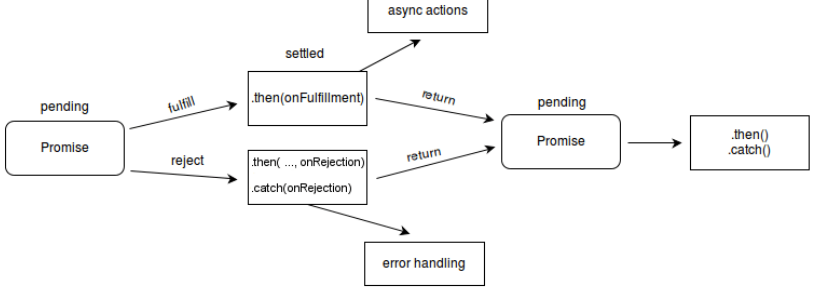
\includegraphics[width=6.26772in,height=1.5in]{media/image7.png}

COMANDI CISCO 5°

Comandi fatti in quinta:

\section{ROUTING STATIC}\label{routing-static}

nella sezione STATIC del router:

\begin{itemize}
\item
  nel Network =\textgreater{} ind. ip dell'altra rete (quella da
  raggiungere);
\item
  nel Mask =\textgreater{} subnet mask della rete da raggiungere;
\item
  nel Next Hop =\textgreater{} l'ind. del router da cui passare.
\end{itemize}

Oppure nella CLI usare il comando:

\textbf{\hl{ip route {[}ind IP{]} {[}mask{]} {[}next hop{]} {[}distanza
amministrativa{]}}}

\emph{La dist. amm. è facoltativa}

In base all'ind. che metto la rotta può essere:

\begin{itemize}
\item
  \textbf{network}: fa match con tutta la rete;
\item
  \textbf{predefinita}: fa match con tutti quelli che non hanno altri
  match;
\item
  \textbf{host}: singolo host.
\end{itemize}

\section{ROUTING SWITCH LAYER 3}\label{routing-switch-layer-3}

\begin{itemize}
\item
  \textbf{\hl{sdm prefer lanbase-routing}}
\item
  \textbf{\hl{reload}}
\item
  \textbf{\hl{ip routing}}
\end{itemize}

\emph{creo la vlan, metto l'ind e mask ed eventualmente la accendo}

\begin{itemize}
\item
  \textbf{\hl{interface vlan {[}nlan{]}}}
\item
  \textbf{\hl{ip address {[}indirizzo{]} {[}mask{]}}}
\item
  \textbf{\hl{no shutdown}}
\end{itemize}

\section{COMANDI TELNET}\label{comandi-telnet}

bisogna sempre fare enable secret ma le password viaggiano in chiaro con
telnet

con SSH invece no. Utile per programmare da lontano lo switch.

\begin{quote}
Comandi base router/switch (in conf t):
\end{quote}

\begin{itemize}
\item
  \textbf{\hl{line vty {[}range porte es. 0 15{]}} nella config verrà
  segnato come line vty 0 4 + line vty 5 15}
\item
  \textbf{\hl{password {[}``password''{]}}}
\item
  \textbf{\hl{login}}
\item
  \textbf{\hl{exit}}
\item
  \textbf{\hl{enable password/secret {[}``password''{]}}}
\end{itemize}

\begin{quote}
Per lo switch con VLAN:
\end{quote}

\begin{itemize}
\item
  \textbf{\hl{interface vlan 1 (vlan di default)}}
\item
  \textbf{\hl{ip address {[}``indirizzo ip della stessa rete ma
  nuovo''{]} {[}mask{]} (come se fosse un host)}}
\item
  \textbf{\hl{no shutdown}}
\item
  \textbf{\hl{line vty {[}range porte{]}}}
\item
  \textbf{\hl{password {[}password{]}}}
\item
  \textbf{\hl{login}}
\item
  \textbf{\hl{exit}}
\item
  \textbf{\hl{ip default-gateway {[}``indirizzo ip''{]}}}
\item
  \textbf{\hl{enable password/secret {[}``password''{]}}}
\end{itemize}

\begin{quote}
Nel laptop nel cmd:
\end{quote}

\begin{itemize}
\item
  \textbf{\hl{telnet {[}IP dello switch messo prima{]}}}
\item
  \textbf{\hl{eventuale password}}
\end{itemize}

\section{COMANDI SSH}\label{comandi-ssh}

Nel router/switch:

\begin{itemize}
\item
  \textbf{\hl{ip domain name {[}nome{]}}}
\item
  \textbf{\hl{hostname {[}nome{]}}}
\item
  \textbf{\hl{crypto key generate rsa}}
\item
  \textbf{\hl{1024 o 512 dipende da quanto sicura è la key}}
\item
  \textbf{\hl{username {[}username{]} password {[}password{]}}
  distinguiamo chi accede, creiamo un user+psw per ogni persona che
  dovrà accedere}
\item
  \textbf{\hl{ip ssh version {[}numero versione (2){]}}}
\item
  \textbf{\hl{line vty 0 15}}
\item
  \textbf{\hl{transport input ssh}}
\item
  \textbf{\hl{login local}}
\end{itemize}

Con \textbf{\hl{show ip ssh}} mostriamo la configurazione

Nel cmd:

\begin{itemize}
\item
  \textbf{\hl{ssh -L {[}username{]} {[}IP (o il nome messo nell'ip
  domain name){]}}}
\end{itemize}

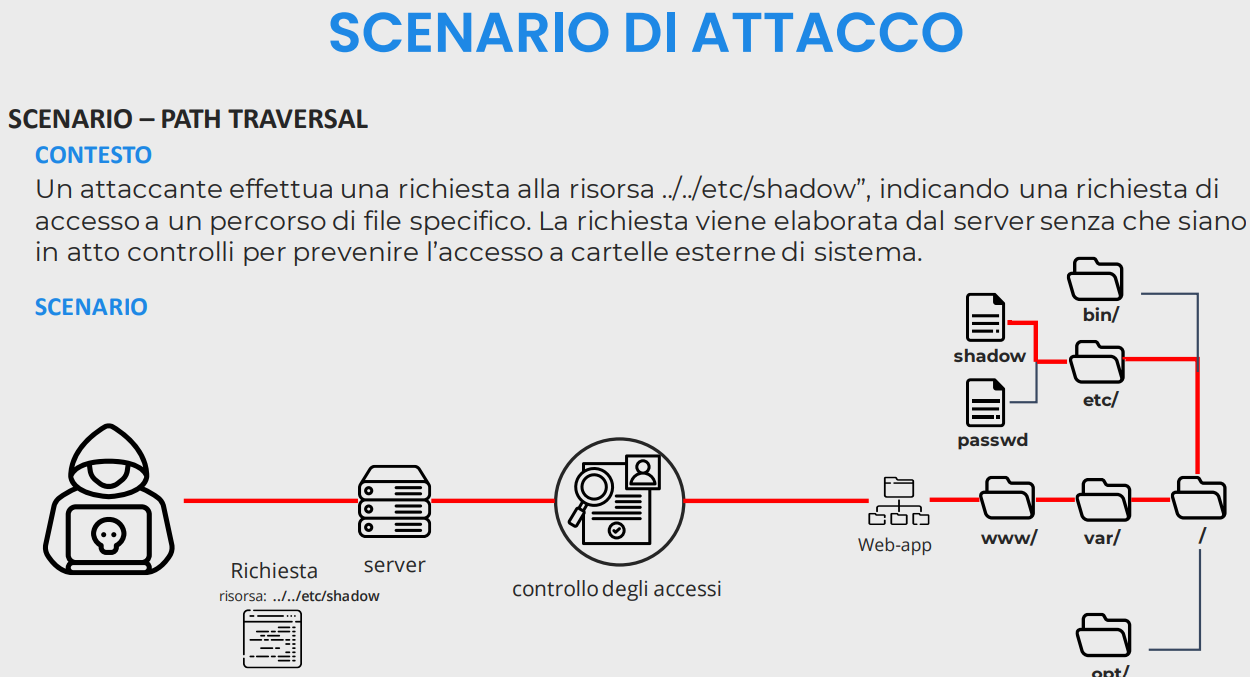
\includegraphics[width=6.89764in,height=2.31637in]{media/image30.png}

\emph{\textbf{\hl{\ul{esempio rete con ssh/telnet}}}}

\section{COMANDI FTP CLIENT E SERVER}\label{comandi-ftp-client-e-server}

Creare tot reti con un server in comune dove andremo a prendere i file;
andare nei services nel server, poi nella sezione FTP e aggiungere un
utente.

Nel cmd per fare upload sul Server:

\begin{itemize}
\item
  \textbf{\hl{ftp {[}indirizzo server{]}}}
\item
  \textbf{\hl{put {[}nome file{]}}}
\end{itemize}

Nel cmd per fare download

\begin{itemize}
\item
  \textbf{\hl{ftp {[}indirizzo server{]}}}
\item
  \textbf{\hl{get {[}nome file{]}}}
\end{itemize}

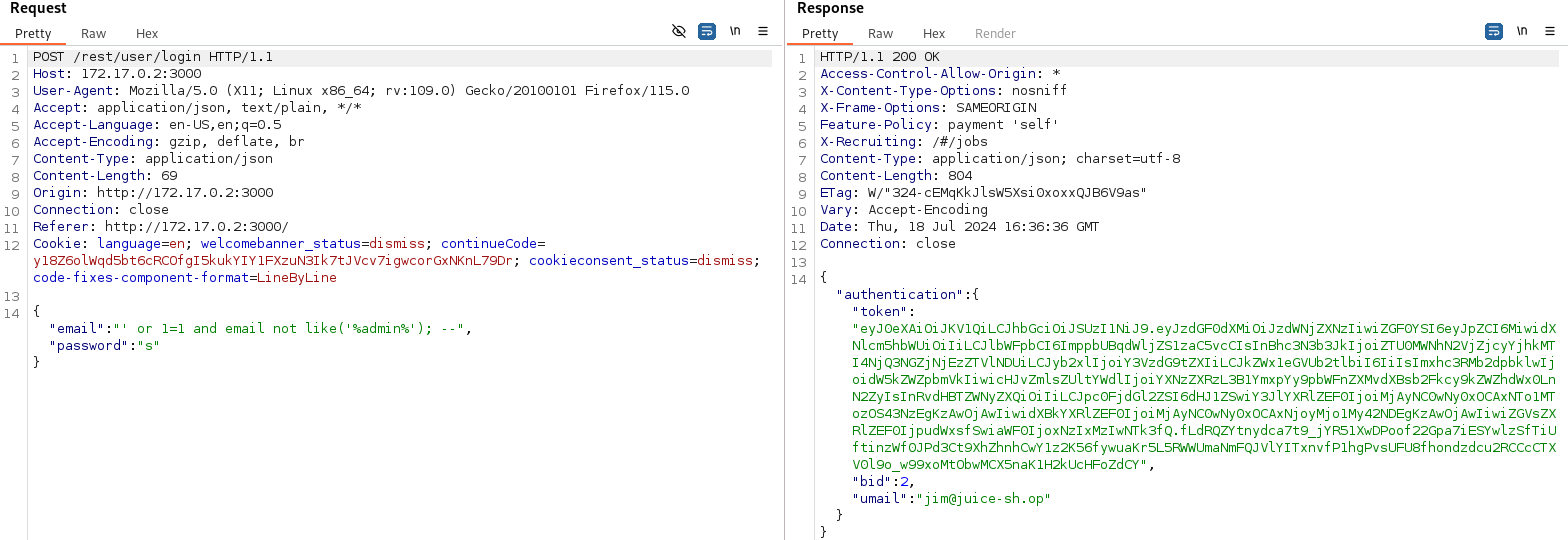
\includegraphics[width=7.07813in,height=3.42708in]{media/image29.png}

\emph{\textbf{\hl{\ul{esempio rete con FTP lato server e RIP}}}}

\section{RIP (Router popolamento)}\label{rip-router-popolamento}

Nei vari router in conf t:

\begin{itemize}
\item
  \textbf{\hl{router rip}}
\item
  \textbf{\hl{version 2}} (La versione con Subnet Mask)
\item
  \textbf{\hl{network {[}ind ip rete1{]}}}
\item
  \textbf{\hl{network {[}ind ip rete2{]}}}
\end{itemize}

(Ripetere network tante quante sono le reti da collegare)

\section{\texorpdfstring{\textbf{DHCP}}{DHCP}}\label{dhcp}

In config: DG

\begin{itemize}
\item
  \textbf{\hl{ip dhcp pool {[}Lan{]}}}
\item
  \textbf{\hl{network {[}indirizzo di rete{]} {[}SM{]}}}
\item
  \textbf{\hl{default-router {[}ind router{]}}}
\item
  \hl{\textbf{ip dhcp excluded-address {[}indirizzo{]}} (per non far
  inserire a dhcp alcuni indirizzi)}
\end{itemize}

Successivamente nel PC possiamo fare \textbf{\hl{ip address dhcp}} per
assegnare uno degli indirizzi nel pool nella macchine

\section{COMANDI FIREWALL E ACL}\label{comandi-firewall-e-acl}

ACL STANDARD SENZA ACCESSO ALLE PORTE

In config: DG

\begin{itemize}
\item
  \hl{\textbf{access-list {[}numero lista es.1{]} {[}deny/permit{]}
  {[}indirizzo{]} {[}wildcard ovvero il NOT della subnetmask
  (255.255.255.0 → 0.0.0.255)} dice se vado a isolare una rete o un
  \textbf{host (0.0.0.0){]}}}
\item
  \textbf{Esempio1 =\textgreater{}} \textbf{access list 1 permit any}
  (per consentire a tutti di comunicare).
\item
  \textbf{Esempio2 =\textgreater{}} \textbf{access list 1 permit
  192.168.2.0 0.0.0.255}(permette alla LAN con quell'indirizzo di rete
  di comunicare).
\item
  Bisogna specificare dove si applicano queste regole: scegliamo
  l'interfaccia di output con: \textbf{\hl{interface {[}interfaccia{]}}}
\item
  \hl{\textbf{ip access-group {[}numero lista{]} {[}in/out{]}} si
  sceglie \textbf{in} se l'ACL deve essere applicata su un host
  all'interno della LAN, al contrario si sceglie \textbf{out}}
\end{itemize}

ACL ESTESE

\begin{itemize}
\item
  \textbf{\hl{access-list {[}numero lista es.101{]} {[}deny/permit{]}
  {[}protocollo{]} host {[}indirizzo mittente{]} host {[}indirizzo
  destinatario{]} eq {[}numero porta lv7{]}}}
\item
  \textbf{Esempio1 =\textgreater{}} \textbf{access-list 101 permit tcp
  host 192.168.2.1 host 192.168.1.100 eq 80} (il PC con ind. 192.168.2.1
  può comunicare con il server 192.168.1.100 sulla porta 80)
\item
  \hl{\textbf{access-list {[}numero lista{]} deny ip any any} (per
  negare tutti gli altri tipi di traffico)}
\item
  \hl{aggiungere la lista all'interfaccia come nel passo per le acl
  standard}
\end{itemize}

ACL NAMED

\begin{itemize}
\item
  \textbf{\hl{ip access-list {[}standard/extended{]} {[}name{]}}}
  -\textgreater{} dopo questo comando tutte le acl fatte saranno già nel
  gruppo {[}name{]}.
\end{itemize}

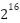
\includegraphics[width=6.26772in,height=2.05556in]{media/image3.png}

\section{NAT STATICO}\label{nat-statico}

In config: DG

Sezione inside(da nascondere) da cui arriva il traffico e sezione
outside.

\begin{itemize}
\item
  \hl{Scegliere l'interfaccia inside \textbf{(interface
  {[}interfaccia{]})}}
\item
  \hl{\textbf{ip nat inside}(nella interfaccia della sezione inside)}
\item
  \hl{exit}
\item
  \hl{Scegliere l'interfaccia outside \textbf{(interface
  {[}interfaccia{]})}}
\item
  \hl{\textbf{ip nat outside}(nella interfaccia della sezione esterna)}
\item
  \hl{\textbf{ip nat inside source static {[}ip del computer
  dell'inside{]} {[}ip pubblico che assegniamo in maniera statica{]}}
  (sempre nella interfaccia dell'outside)}
\item
  \textbf{Esempio1 =\textgreater{}} ip nat inside source static
  192,168,1,1 200.100.50.254
\item
  \hl{\textbf{do wr} (per applicare la conf. al router, da fare in
  config)}
\item
  \hl{per vedere il corretto funzionamento fare una request http dal
  browser e usare la simulation}
\end{itemize}

\section{NAT DINAMICO}\label{nat-dinamico}

\begin{itemize}
\item
  \textbf{\hl{ip nat pool {[}nome pool{]} {[}indirizzo pubblico di
  partenza pool{]} {[}indirizzo pubblico di fine pool{]} netmask
  {[}SM{]}}}
\item
  \textbf{Esempio1 =\textgreater{}} ip nat pool nomePool 200.100.50.1
  200.100.50.10 255.255.255.0
\item
  \textbf{\hl{access-list 10 permit {[}rete{]} {[}SM al contrario{]}}}
\item
  \textbf{Esempio2 =\textgreater{}} access-list 10 permit 192.168.1.0
  0.0.0.255
\item
  \textbf{\hl{ip nat inside source list {[}source access list{]} pool
  {[}nomepool{]}}}
\item
  \textbf{Esempio3 =\textgreater{}} ip nat inside source list 10 pool
  internetworking
\item
  \hl{Scegliere l'interfaccia inside \textbf{(interface
  {[}interfaccia{]})}}
\item
  \hl{\textbf{ip nat inside}(nella interfaccia della sezione inside)}
\item
  \hl{exit}
\item
  \hl{Scegliere l'interfaccia outside \textbf{(interface
  {[}interfaccia{]})}}
\item
  \hl{\textbf{ip nat outside}(nella interfaccia della sezione esterna)}
\item
  \hl{exit}
\item
  \hl{\textbf{do wr} (per applicare la conf. al router, da fare in
  config)}
\end{itemize}

\section{PROTOCOLLI}\label{protocolli}

\begin{longtable}[]{@{}
  >{\raggedright\arraybackslash}p{(\linewidth - 4\tabcolsep) * \real{0.3333}}
  >{\raggedright\arraybackslash}p{(\linewidth - 4\tabcolsep) * \real{0.3333}}
  >{\raggedright\arraybackslash}p{(\linewidth - 4\tabcolsep) * \real{0.3333}}@{}}
\toprule\noalign{}
\begin{minipage}[b]{\linewidth}\centering
\hl{Nome}
\end{minipage} & \begin{minipage}[b]{\linewidth}\centering
\hl{Porta}
\end{minipage} & \begin{minipage}[b]{\linewidth}\centering
\hl{TCP o UDP}
\end{minipage} \\
\begin{minipage}[b]{\linewidth}\raggedright
\hl{HTTP/HTTPS}
\end{minipage} & \begin{minipage}[b]{\linewidth}\raggedright
\hl{80/443}
\end{minipage} & \begin{minipage}[b]{\linewidth}\raggedright
\hl{TCP}
\end{minipage} \\
\begin{minipage}[b]{\linewidth}\raggedright
\hl{DHCP}
\end{minipage} & \begin{minipage}[b]{\linewidth}\raggedright
\hl{68(client)/67(server)}
\end{minipage} & \begin{minipage}[b]{\linewidth}\raggedright
\hl{UDP}
\end{minipage} \\
\begin{minipage}[b]{\linewidth}\raggedright
\hl{FTP}
\end{minipage} & \begin{minipage}[b]{\linewidth}\raggedright
\hl{21(comandi) e 20(dati)}
\end{minipage} & \begin{minipage}[b]{\linewidth}\raggedright
\hl{TCP}
\end{minipage} \\
\begin{minipage}[b]{\linewidth}\raggedright
\hl{DNS}
\end{minipage} & \begin{minipage}[b]{\linewidth}\raggedright
\hl{53}
\end{minipage} & \begin{minipage}[b]{\linewidth}\raggedright
\hl{UDP/TCP}
\end{minipage} \\
\begin{minipage}[b]{\linewidth}\raggedright
\hl{SMTP}
\end{minipage} & \begin{minipage}[b]{\linewidth}\raggedright
\hl{25}
\end{minipage} & \begin{minipage}[b]{\linewidth}\raggedright
\hl{TCP}
\end{minipage} \\
\begin{minipage}[b]{\linewidth}\raggedright
\hl{POP3}
\end{minipage} & \begin{minipage}[b]{\linewidth}\raggedright
\hl{110}
\end{minipage} & \begin{minipage}[b]{\linewidth}\raggedright
\hl{TCP}
\end{minipage} \\
\midrule\noalign{}
\endhead
\bottomrule\noalign{}
\endlastfoot
\end{longtable}

COMANDI FATTI ALLA VEM

\section{AAA}\label{aaa}

Se in una azienda sono presenti innumerevoli device con utenti replicati
su ognuno, è possibile adottare un server per l'autenticazione.

\emph{``Authentication, authorization, and accounting (AAA) server''}

Vediamo come configurare uno switch (in config) se è presente un server
AAA RADIUS:

\begin{itemize}
\item
  \textbf{\hl{aaa new-model}}
\item
  \textbf{\hl{radius-server host {[}IP AAA {]} key {[}key{]}}}
\item
  \textbf{\hl{aaa authentication login default group radius local} lista
  di metodi di autenticazione (group radius e local)}
\item
  \textbf{\hl{line vty 0 5}}
\item
  \textbf{\hl{login authentication default}}
\end{itemize}

\section{Address table}\label{address-table}

\textbf{Nello switch:}

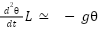
\includegraphics[width=5.5951in,height=3.04849in]{media/image31.png}

\textbf{Nel router:}

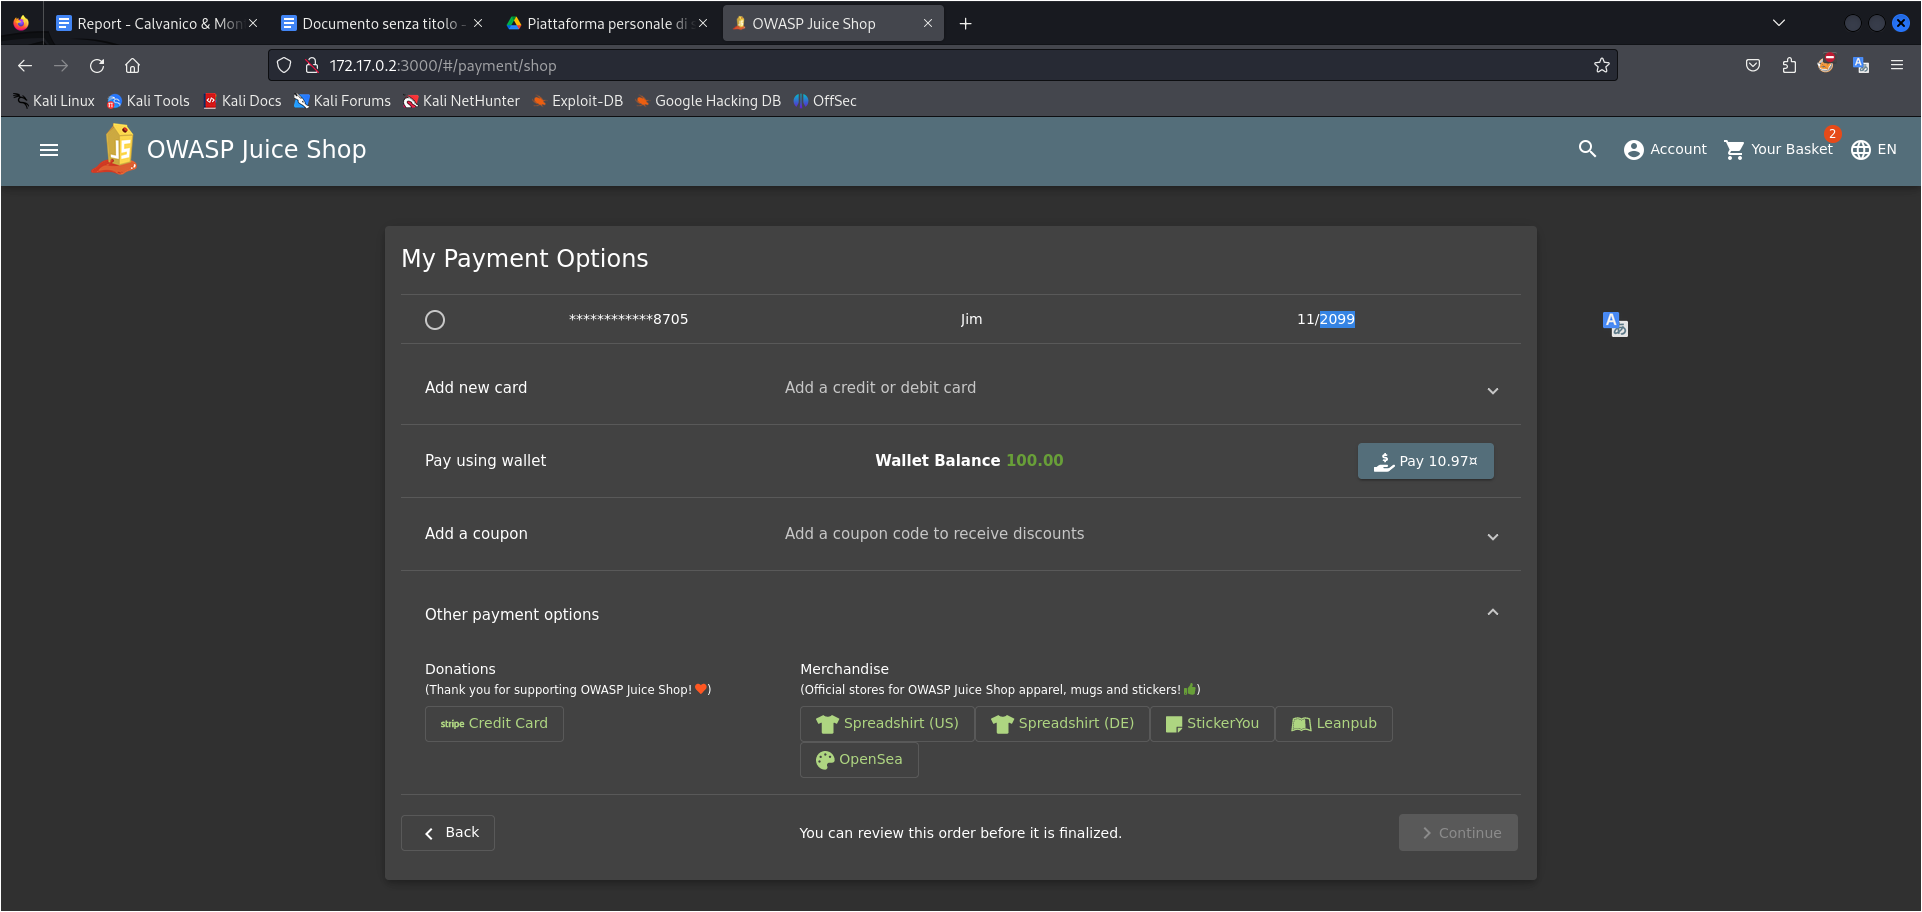
\includegraphics[width=6.26772in,height=1.33333in]{media/image12.png}

\section{Interfaces configuration}\label{interfaces-configuration}

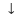
\includegraphics[width=6.00521in,height=2.19459in]{media/image23.png}

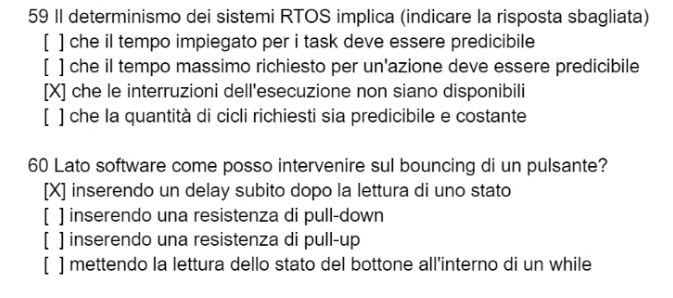
\includegraphics[width=6.26772in,height=4.625in]{media/image21.png}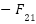
\includegraphics[width=6.26772in,height=4.26389in]{media/image14.png}

Il comando \textbf{\hl{show interfaces}} restituisce tanti valori nel
dettaglio:

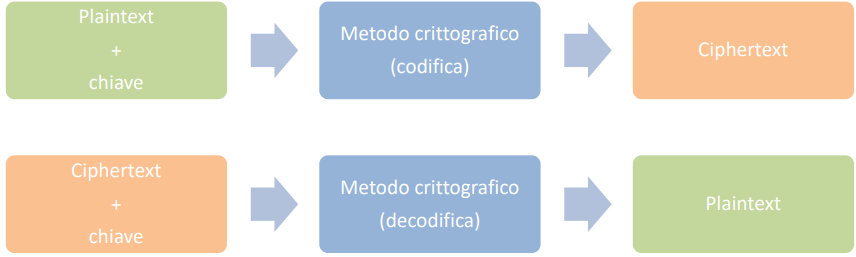
\includegraphics[width=6.26772in,height=3.34722in]{media/image19.png}

\section{VTP - VLAN Trunking
Protocol}\label{vtp---vlan-trunking-protocol}

Serve per propagare in automatico uno VLAN in ogni switch della rete
senza doverle inserire manualmente in ciascuna.

Ogni switch può assumere una modalità:

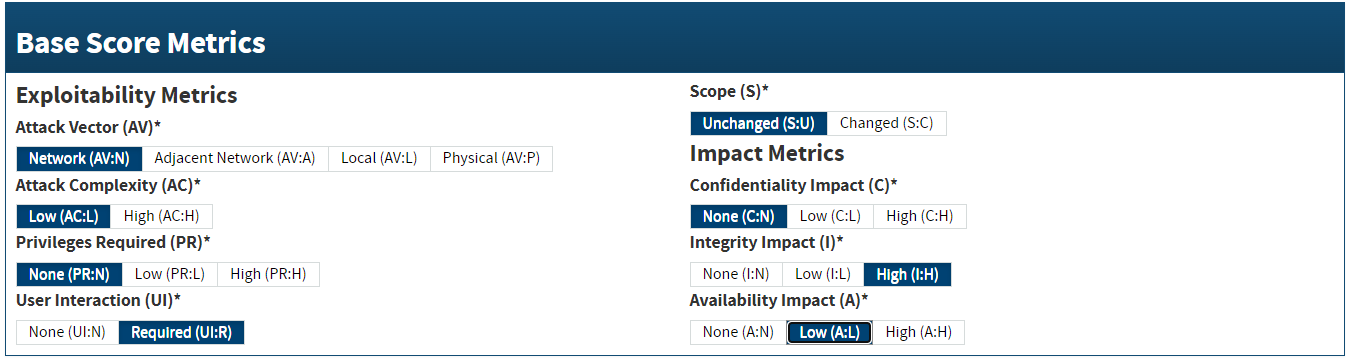
\includegraphics[width=6.26772in,height=1.61111in]{media/image26.png}

\emph{Gli switch server possono coesistere}

Negli switch server ogni volta che modifichiamo il database delle VLAN
il revision number aumenta e le VLAN vengono propagate in base dallo
switch (anche se non in server mode) con il revision number più grande.

\emph{Se aggiungo uno switch alla rete con un revision number sbagliato
introduco degli errori nelle tabelle degli altri switch, questo switch
sbagliato si chiama \textbf{VTP BOMB}}

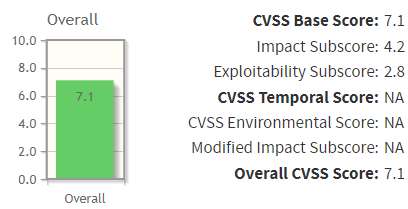
\includegraphics[width=5.38866in,height=1.38415in]{media/image27.png}

\textbf{\hl{show vtp status} -\textgreater{}} monitoriamo il
funzionamento.

Il VTP Pruning migliora le prestazioni di rete diminuendo il traffico
non necessario, andando a bloccare frame broadcast verso VLAN che non
hanno interesse in quel messaggio.

\section{STP/RSTP}\label{stprstp}

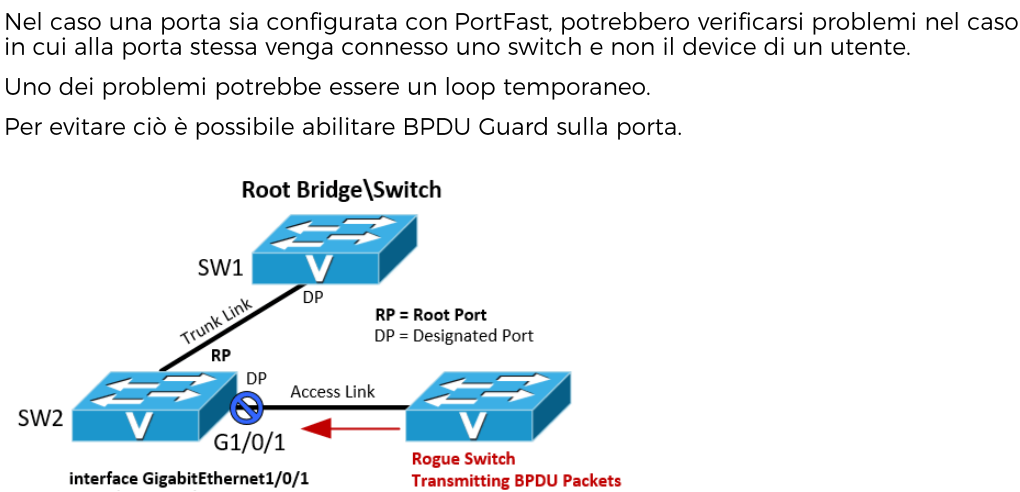
\includegraphics[width=6.26772in,height=1.11111in]{media/image15.png}

Essendo su apparati Cisco usiamo i loro protocolli che funzionano in
ugual modo a STP/RSTP/MSTP.

Si può inserire una priorità ad ogni switch per decidere quale diventerà
lo switch root.

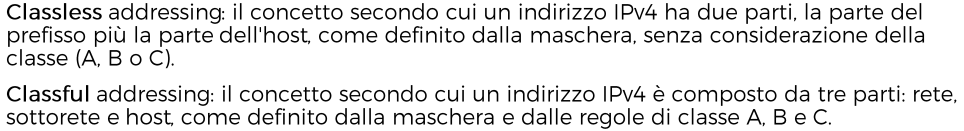
\includegraphics[width=6.26772in,height=0.70833in]{media/image6.png}

Elenco di comandi:

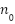
\includegraphics[width=6.26772in,height=3.65278in]{media/image17.png}

\begin{itemize}
\item
  \textbf{\hl{show spanning-tree}} =\textgreater{} mostro tutti i
  dettagli
\end{itemize}

\section{PortChannel/EtherChannel}\label{portchanneletherchannel}

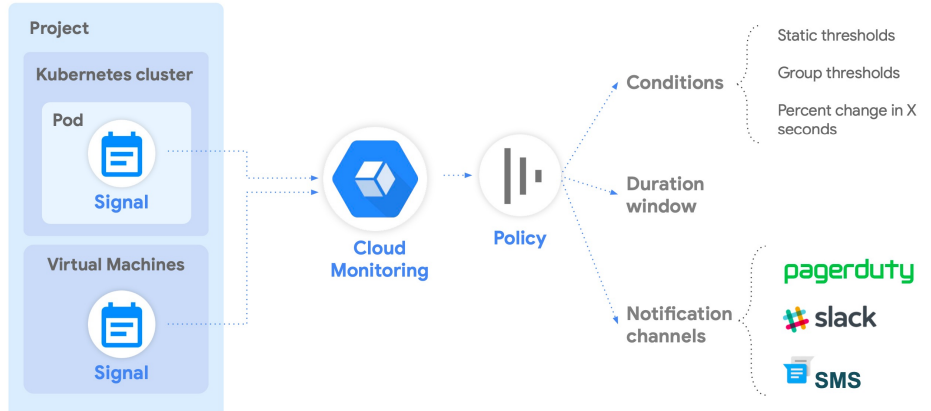
\includegraphics[width=6.26772in,height=5.16667in]{media/image28.png}

In questo modo STP contera i due canali come uno unico e in caso di
guasti non si bloccherà tutto.

Per far funzionare il PortChannel le porte devono essere uguali, nel
dettaglio:

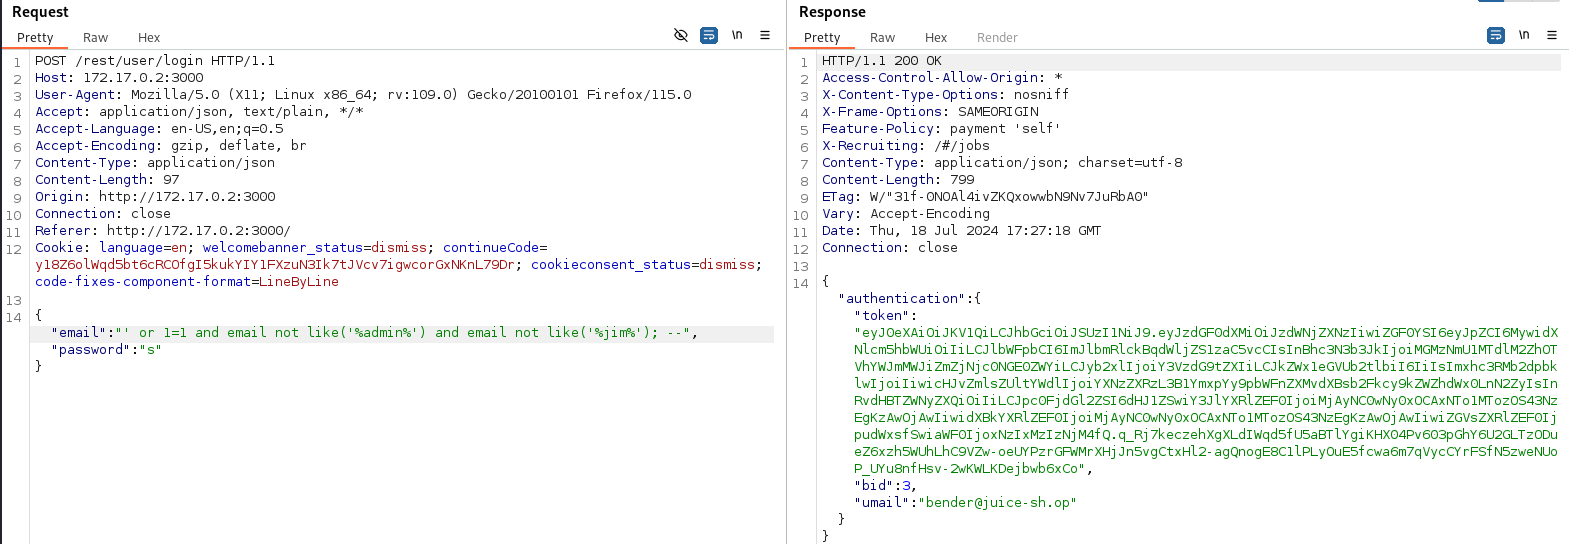
\includegraphics[width=4.57813in,height=1.31564in]{media/image16.png}

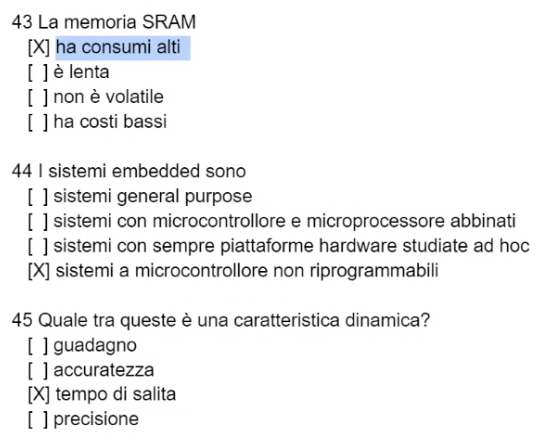
\includegraphics[width=4.88385in,height=2.57113in]{media/image8.png}

Con questo metodo decidiamo che il traffico verrà bilanciato su tutti i
canali in base a determinati vincoli.

\section{Root Guard}\label{root-guard}

Diciamo che una certa interfaccia eviti i problemi che senza root guard
si verificherebbero all\textquotesingle inserimento di un nuovo switch:

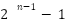
\includegraphics[width=5.00521in,height=0.55706in]{media/image10.png}

\section{BPDU Guard}\label{bpdu-guard}

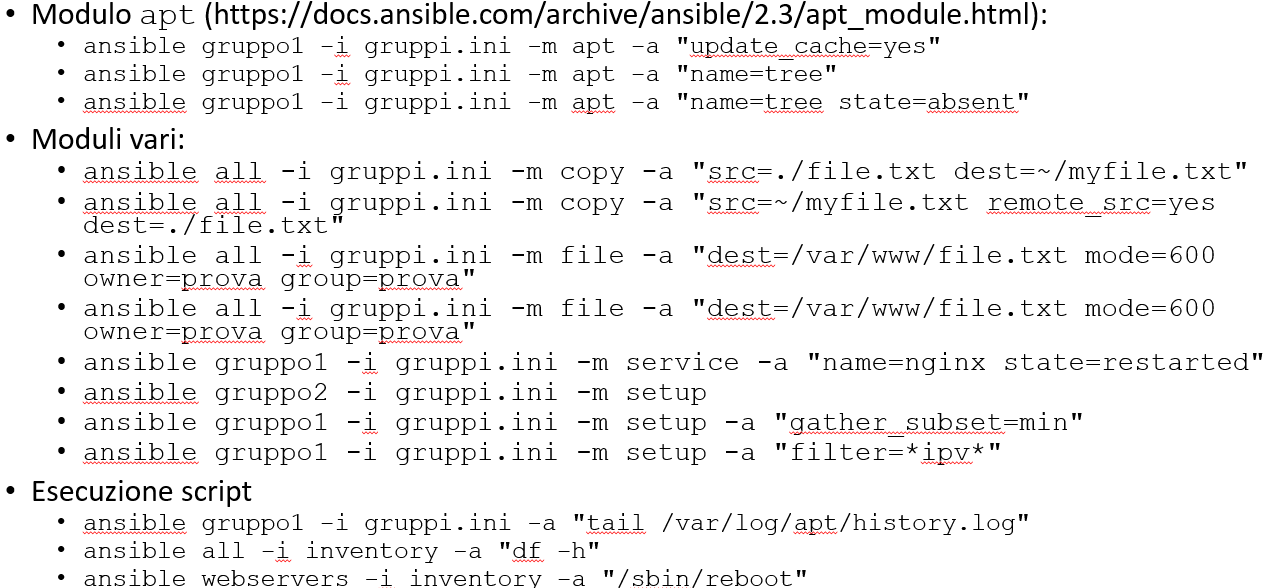
\includegraphics[width=4.47917in,height=1.90625in]{media/image2.png}

\section{OSPF}\label{ospf}

\subsection{Single Area}\label{single-area}

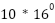
\includegraphics[width=6.26772in,height=3.45833in]{media/image24.png}

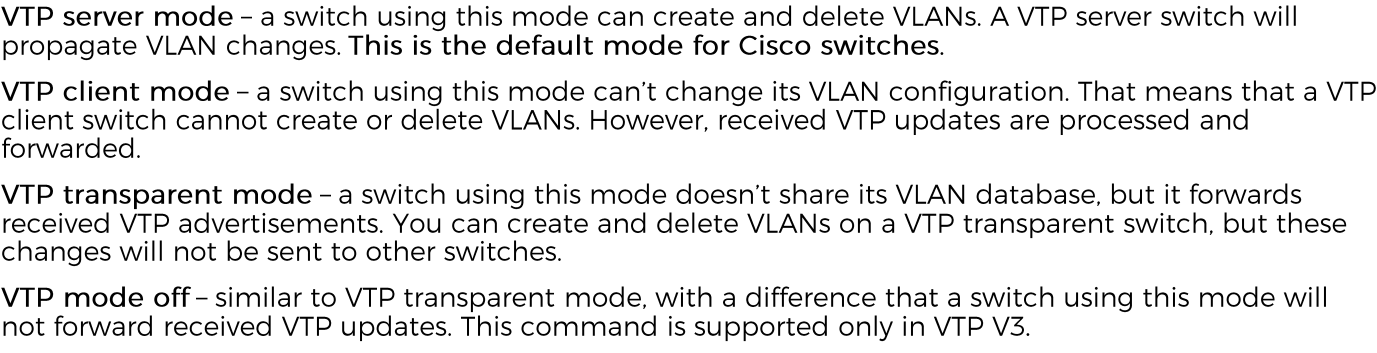
\includegraphics[width=6.26772in,height=3.65278in]{media/image22.png}

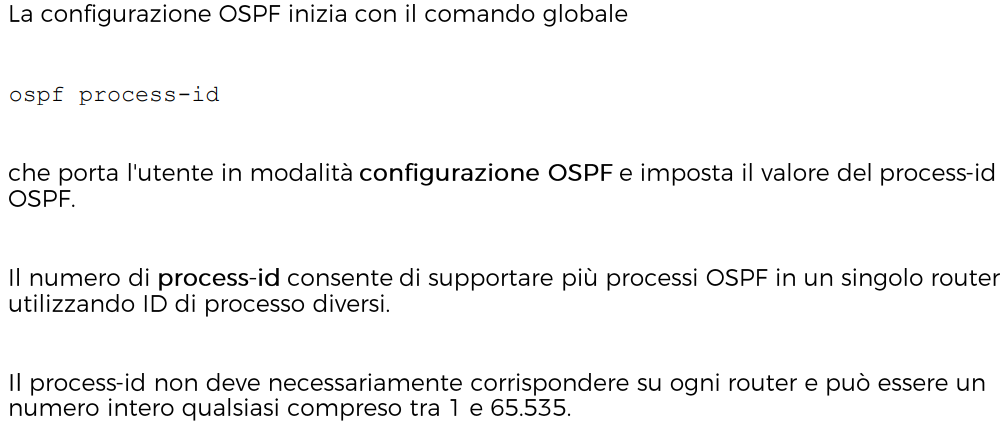
\includegraphics[width=6.26772in,height=2.63889in]{media/image4.png}

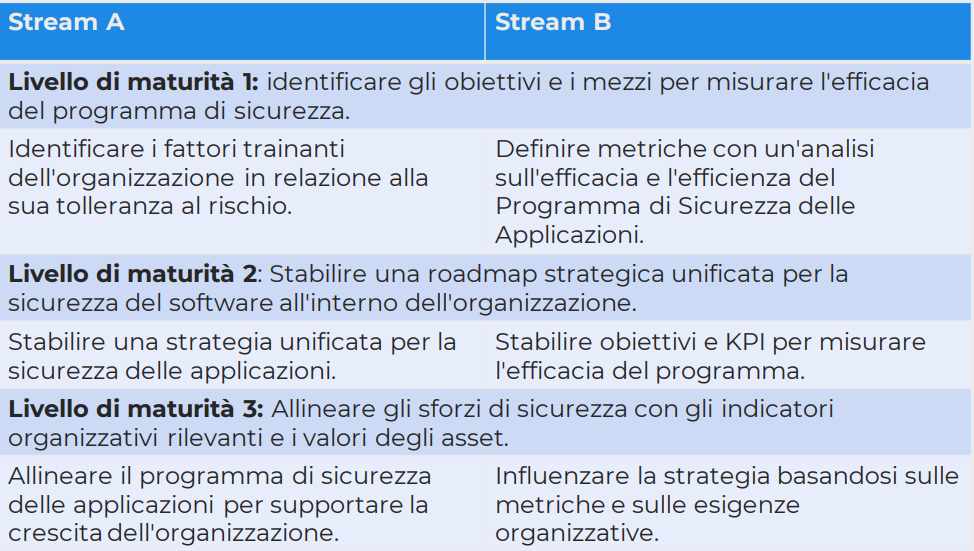
\includegraphics[width=6.26772in,height=2.02778in]{media/image13.png}

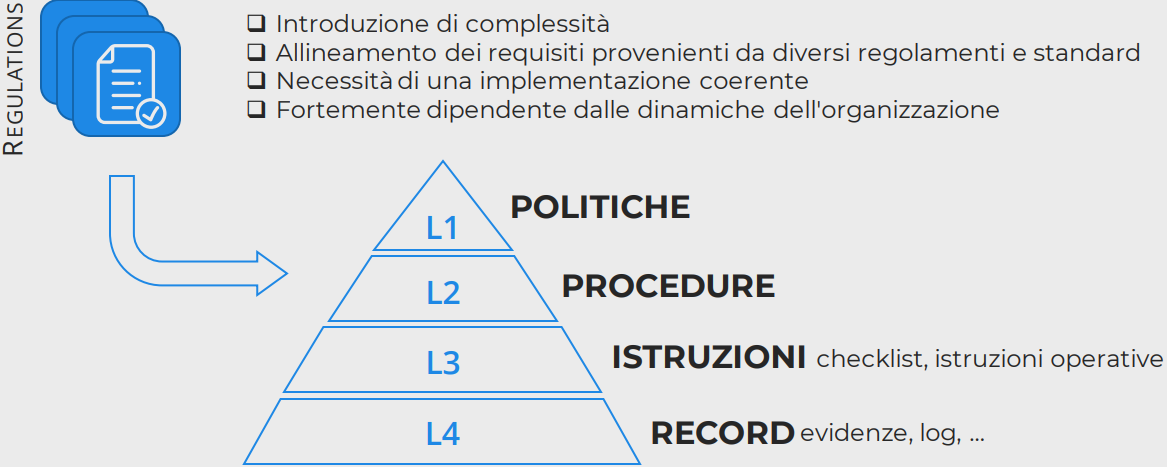
\includegraphics[width=6.26772in,height=1.86111in]{media/image18.png}

La configurazione degli altri router (R3/4) è simile cambiano gli
indirizzi e le network

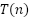
\includegraphics[width=2.76794in,height=2.15104in]{media/image5.png}

All'invio del primo comando ci uscirà una tabella con una sezione State,
questi sono gli stati disponibili:

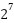
\includegraphics[width=6.26772in,height=1.76389in]{media/image11.png}

\subsection{Multi area}\label{multi-area}

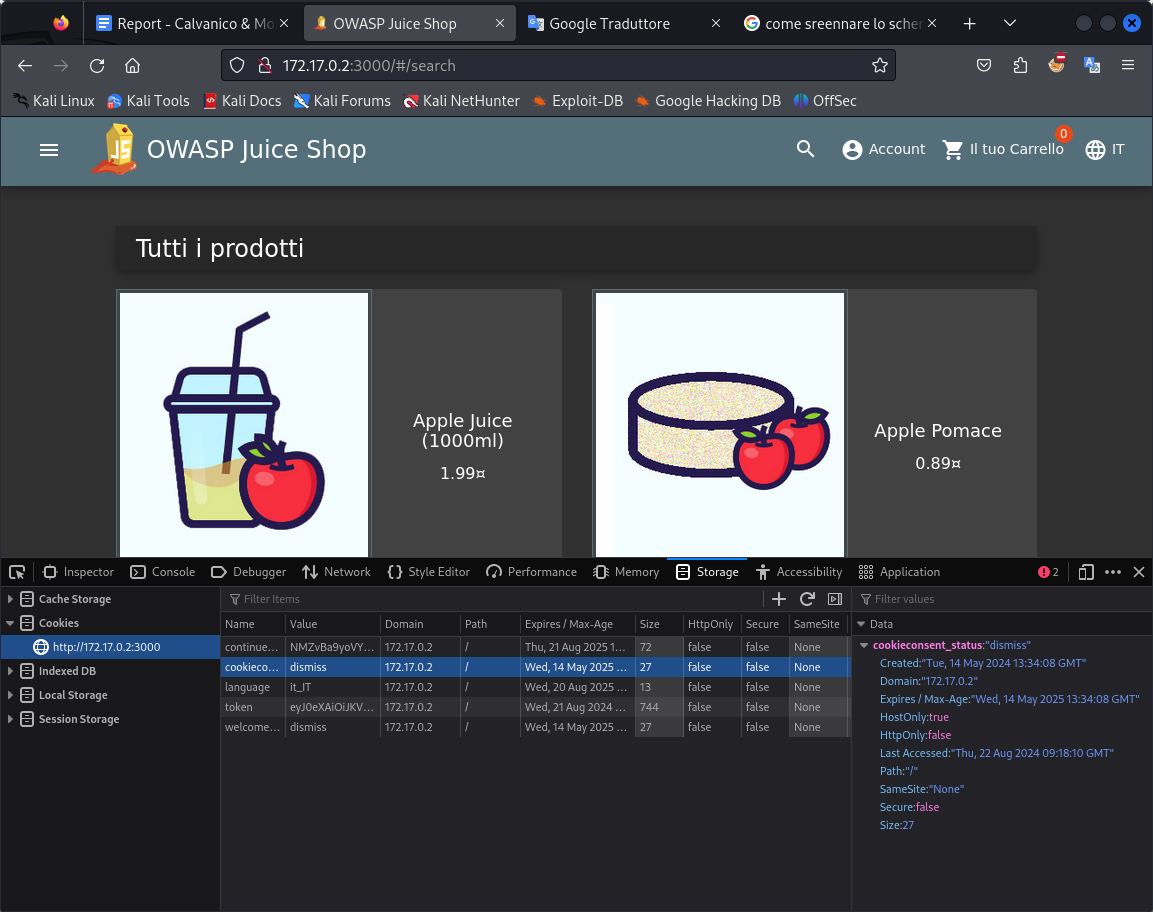
\includegraphics[width=6.26772in,height=3.52778in]{media/image25.png}

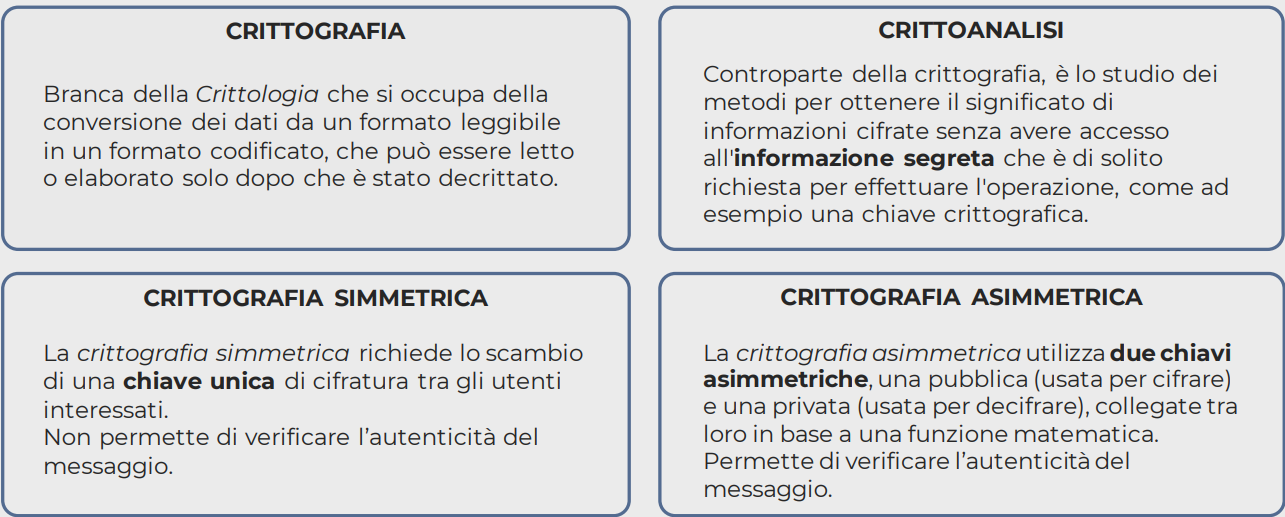
\includegraphics[width=6.26772in,height=1.31944in]{media/image20.png}

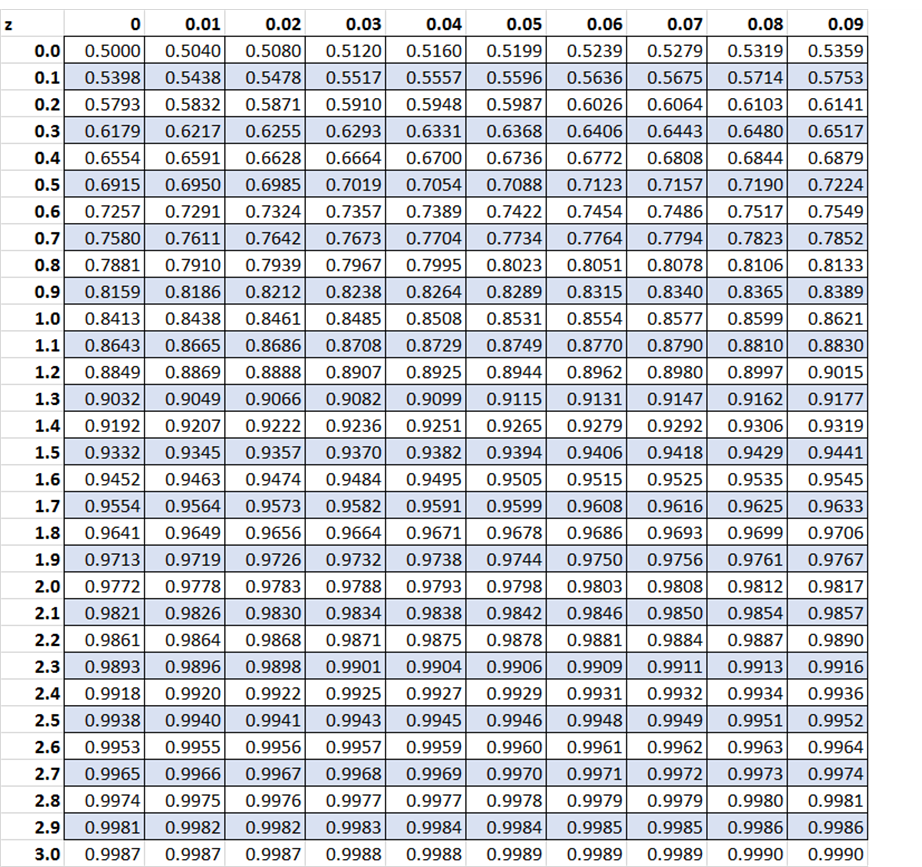
\includegraphics[width=6.26772in,height=2.84722in]{media/image9.png}

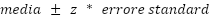
\includegraphics[width=6.26772in,height=3.54167in]{media/image1.png}

\section{Vari}\label{vari}

\begin{itemize}
\item
  \textbf{\hl{logging synchronous}}: dice allo switch di aspettare che
  finiamo di scrivere prima di inviare log
\item
  \textbf{\hl{history size {[}numero{]}}}: indica quanti comandi la
  history tiene traccia
\item
  \textbf{\hl{exec-timeout {[}minuti{]}}}: indica quanto tempo l'utente
  può rimanere inattivo prima di essere kickato
\end{itemize}

\textbf{CONFIGURAZIONE WIRELESS}

\subsubsection{\texorpdfstring{\textbf{PRIMO PASSO: config del router
WI-FI}}{PRIMO PASSO: config del router WI-FI}}\label{primo-passo-config-del-router-wi-fi}

\begin{itemize}
\item
  Scegliamo il router WRT300N;
\item
  Clicchiamo sull'apparato e \textbf{selezioniamo GUI}, andiamo in
  \textbf{Setup → Basic Setup} e andiamo in \textbf{Network Setup};
\item
  Qui scegliamo la configurazione degli indirizzi che vogliamo (l'ip del
  router wireless farà da DG per i dispositivi mobili);
\item
  Terminato il setup salviamo con il bottone \textbf{Save Settings};
\item
  Poi apriamo \textbf{Wireless → Basic Wireless Settings} e impostiamo
  l'SSID con un nome a nostra scelta e salviamo;
\item
  Ora apriamo la scheda \textbf{Wireless → Wireless Security} e
  impostiamo:

  \begin{itemize}
  \item
    la protezione \textbf{WPA2-Enterprise} con crittografia AES;
  \item
    l'indirizzo IP del server RADIUS: uno della stessa rete del router;
  \item
    la Shared Secret.
  \end{itemize}
\item
  Dopo aver salvato la configurazione router è terminata.
\end{itemize}

\subsubsection{\texorpdfstring{\textbf{SECONDO PASSO: config del server
AAA}}{SECONDO PASSO: config del server AAA}}\label{secondo-passo-config-del-server-aaa}

\begin{itemize}
\item
  Scegliamo un server e nei \textbf{Services} scegliamo il AAA e
  impostiamo nella \textbf{Network Configuration}:

  \begin{itemize}
  \item
    come Client Name l'SSID della rete wireless;
  \item
    come Client IP l'ind IP del router wireless;
  \item
    come Secret la Shared Secret impostata sul router wireless;
  \item
    come Service Type selezioniamo RADIUS.
  \end{itemize}
\end{itemize}

\begin{quote}
ora con \textbf{ADD} aggiungiamo la configurazione creata;
\end{quote}

\begin{itemize}
\item
  Nella parte sotto (\textbf{User Setup}) configuriamo le tot. utenze
  previste e clicchiamo \textbf{ADD} per aggiungerle.
\end{itemize}

\hl{}

\subsubsection{\texorpdfstring{\textbf{TERZO PASSO: config dei
dispositivi
wireless}}{TERZO PASSO: config dei dispositivi wireless}}\label{terzo-passo-config-dei-dispositivi-wireless}

\begin{itemize}
\item
  Clicchiamo nel dispositivo scelto andiamo in \textbf{Physical} lo
  spegniamo e cambiamo il modulo Ethernet con uno wireless
  (\textbf{WMP300N}) e lo riaccendiamo;
\item
  In \textbf{Config} selezioniamo Wireless0 e impostiamo:

  \begin{itemize}
  \item
    come SSID quello che abbiamo impostato del AAA e nel router;
  \item
    come metodo di Authentication la \textbf{WPA2} specificando le
    credenziali;
  \item
    e come Encryption Type \textbf{AES}.
  \end{itemize}
\item
  Questa configurazione è da fare per ogni dispositivo della rete
  wireless.
\end{itemize}

\textbf{MACCHINE VIRTUALI}

Prerequisiti Macchine Virtuali (Vanno fatti in entrambe le macchine):

\begin{itemize}
\item
  Macchina → Impostazioni → Rete
\item
  Impostare la rete a ``Rete interna'', lasciare intnet come nome.
\item
  Configurare gli IP delle due macchine.
\item
  Verificare il ping tra le due.
\end{itemize}

Procedimento XAMPP

La sigla ci dice che l\textquotesingle ambiente che stiamo creando è un
ambiente server con particolari caratteristiche: è un server APACHE
(utilizza MariaDB, PhP e Perl);

X: sta ad indicare che è multipiattaforma;

A: ci dice apache;

M: tipo di database su cui fare le operazioni come mariaDB;

P: PHP;

P: Perl è un linguaggio;

Apache se facciamo start creeremo un server web in locale.

se facciamo start in MySQL avremo un database.

Infine attiveremo FileZilla e useremo FTP

C:\textbackslash XAMPP\textbackslash HTdocs (c'è la pagina web) → al
posto del file index.php creare un file index.html. Questa è la nostra
pagina

Per consultare il proprio server nella barra dell'URL di un browser
scrivere 127.0.0.1 oppure localhost/ o anche l'indirizzo IP della
macchina

Creare un nuovo index.html si può scorrere anche dentro le cartelle VA
MESSO IL NOME DOPO LA BARRA.

Procedimento FileZilla

FileZilla: FTP server.

\begin{itemize}
\item
  Andiamo su admin; metti password admin dentro XAMPP
\item
  Edit setting e mettiamo 0 in tutti timeout i timeout dalle
  impostazioni dell'admin da XAMPP
\end{itemize}

per collegarci da un client dobbiamo creare un utente.

\begin{itemize}
\item
  edit → users → add e password
\item
  Shared folders → ADD → mettiamo la cartella che vogliamo condividere
\end{itemize}

abilita tutto

\begin{itemize}
\item
  Avviamo Filezilla client mettiamo host: 127.0.0.1 (Se non usiamo due
  macchine diverse) Nome utente: nome dato alla user e password porta
  lasciarla vuota
\end{itemize}

\section{Configurazione di Rete
Windows}\label{configurazione-di-rete-windows}

\section{Comandi DNS nel cmd}\label{comandi-dns-nel-cmd}

ipconfig /displaydns vediamo il contenuto della cache

ipconfig /flushdns cancelliamo il contenuto della cache

\section{Abilitare connessione desktop remoto
windows}\label{abilitare-connessione-desktop-remoto-windows}

\begin{itemize}
\item
  Pannello di controllo
\item
  Sistema e sicurezza
\item
  Sistema
\item
  Impostazioni di connessione remota (a sinistra)
\item
  Fare la spunta su ``Consenti connessioni di Assistenza remota al
  computer''
\item
  Avanzate:
\item
  fare la spunta su ``Consenti il controllo del computer da postazioni
  remote''
\item
  Ok
\item
  Selezionare ``Consenti connessioni remote al computer''. (In basso)
\end{itemize}

\textbf{SUBNETTING}

\begin{enumerate}
\def\labelenumi{\arabic{enumi})}
\item
  Trovare i bit per sottoreti e per host, per i bit della sottorete fare
  2\textsuperscript{n} \textgreater= del numero di sottoreti ( l' n sarà
  i bit), per gli host prendo la sottorete con più host e faccio
  2\textsuperscript{n} \textgreater= del numero massimo di host -3 ( l'
  n sarà i bit);
\item
  Faccio la somma dei due bit trovati e con la somma trovo la classe che
  devo usare andando a vedere i bit dedicati agli host (Classe A = 24,
  Classe B = 16, Classe C = 8), distribuisco eventuali bit restanti (
  facendo la somma dei bit trovati meno bit degli host di ogni classe e
  andando a scegliere una combinazione);
\item
  Prendiamo la combinazione scelta nel passaggio precedente ( Es. 9+7
  con classe B) e decidiamo un indirizzo, preso a caso, della classe
  scelta (Es. 172.16.0.0), iniziamo facendo al subnet mask andando a
  prendere quella della classe scelta (Es. classe B =\textgreater{}
  255.255.0.0) e mettiamo a 1 tutti i bit della rete ottenendo così la
  subnet mask (Es. 255.255.255.128 =\textgreater{} 111111111 \textbar{}
  0000000).
\end{enumerate}

\begin{quote}
Per gli indirizzi degli host prendiamo il numero dell'host (Es. 30) e il
numero della sottorete (Es. 4° sottorete) e dividiamo così:

172.16.1.158 =\textgreater{} 000000011 \textbar{} 0011110 Nella parte
sinistra dove ci sono i bit della rete metto il numero della sottorete
-1 in binario, in quella a destra dove ci sono i bit destinati agli host
metto il numero dell'host in binario.

Per il D.G. metto a 1 tutti i bit dedicati agli host tranne l'ultimo che
resta 0
\end{quote}

(Es.1 =\textgreater{} 172.16.0.126 =\textgreater{} 00000000 \textbar{}
1111110 Lo 0 finale nella parte a sinistra perchè 1° sottorete.

Es.2 =\textgreater{} 172.16.0.254 =\textgreater{} 00000001 \textbar{}
1111110 L' 1 finale nella parte a sinistra perchè 2° sottorete.)
